\documentclass{ExcelAtFIT}
%\documentclass[czech]{ExcelAtFIT} % when writing in CZECH
%\documentclass[slovak]{ExcelAtFIT} % when writing in SLOVAK


\usepackage{color, colortbl}
\usepackage{siunitx}

%--------------------------------------------------------
%--------------------------------------------------------
%	REVIEW vs. FINAL VERSION
%--------------------------------------------------------

%   LEAVE this line commented out for the REVIEW VERSIONS
%   UNCOMMENT this line to get the FINAL VERSION
\ExcelFinalCopy


%--------------------------------------------------------
%--------------------------------------------------------
%	PDF CUSTOMIZATION
%--------------------------------------------------------

\hypersetup{
	pdftitle={Performance Testing and Analysis of Qpid-Dispatch router},
	pdfauthor={Jakub Stejskal},
	pdfkeywords={Performance Testing, performance analysis, Qpid-Dispatch, router, network technologies}
}

%--------------------------------------------------------
%--------------------------------------------------------
%	ARTICLE INFORMATION
%--------------------------------------------------------

\ExcelYear{2018}

\PaperTitle{Performance Testing and Analysis of Qpid-Dispatch router}

\Authors{Jakub Stejskal*}
\affiliation{*%
  \href{mailto:xstejs24@studfit.vutbr.cz}{xstejs24@stud.fit.vutbr.cz},
  \textit{Faculty of Information Technology, Brno University of Technology}}
%%%%--------------------------------------------------------
%%%% in case there are multiple authors, use the following fragment instead
%%%%--------------------------------------------------------
%\Authors{Jindřich Novák*, Janča Dvořáková**}
%\affiliation{*%
%  \href{mailto:xnovak00@stud.fit.vutbr.cz}{xnovak00@stud.fit.vutbr.cz},
%  \textit{Faculty of Information Technology, Brno University of Technology}}
%\affiliation{**%
%  \href{mailto:xdvora00@stud.fit.vutbr.cz}{xdvora00@stud.fit.vutbr.cz},
%  \textit{Faculty of Information Technology, Brno University of Technology}}

\Keywords{Performance Testing --- performance analysis --- Qpid-Dispatch testing --- router testing --- network technologies --- Messaging Performance Tool}

\Supplementary{\href{https://github.com/maestro-performance/maestro-java}{Downloadable Code}}


%--------------------------------------------------------
%--------------------------------------------------------
%	ABSTRACT and TEASER
%--------------------------------------------------------

\Abstract{
The application performance testing has recently become more important during the application development of all kinds. This paper analyzes the fundamentals of performance testing that are commonly used and, in particular, it focuses on performance testing of components used in Messaging systems, especially the AMQ Messaging Broker and Qpid-Dispatch router. Currently used methods for performance testing of these components are primarily focused only on Messaging Broker and are implemented in the Messaging Performance Tool. However, it still lacks support for more broad range of components especially the Qpid-dispatch. In this paper I describe the improvements of the Messaging Performance Tool to enable the performance testing of Qpid-Dispatch and its capabilities in automatic testing. I evaluate the proposed extension and study the performance of Qpid-Dispatch component on several real world case studies.
}

% \Teaser{
% 	\TeaserImage{java.png}
% 	\TeaserImage{messaging.jpg}
% 	\TeaserImage{red_hat.png}
% }



%--------------------------------------------------------
%--------------------------------------------------------
%--------------------------------------------------------
%--------------------------------------------------------
\begin{document}

\startdocument


%--------------------------------------------------------
%--------------------------------------------------------
%	ARTICLE CONTENTS
%--------------------------------------------------------

%--------------------------------------------------------
%--------------------------------------------------------
%--------------------------------------------------------
%--------------------------------------------------------
\section{Introduction}
Good application performance is one of the main goals during the software development. But what makes software performance so important? Software reliability has to be guaranteed by the owner, but with undesirable performance there could be a lot of issues. This can badly influence software behavior and can subsequently cause a significant outflow of consumers, and even brand destruction, financial damage, or loss of trust. These few reasons should be enough to do a proper performance testing before every software release. Especially for large projects where industries guarantee certain level of software behavior and they would not be able to assure it with insufficient performance testing.

In general an application performance is important. However, smooth network application or hardware performance became much more demanded nowadays, since most of the communication is via the Internet.  Obviously when you make a payment using your internet banking you definitely want to have a stable connection to your bank's website without any delay. Network stability is significantly influenced by network components like routers and switches and hence their performance should be under utmost case. We refer to network performance testing as measurement of network service quality which is directly influenced by \emph{bandwidth, throughput, latency}, etc.

For performance testing of particular network messaging system developed by \emph{Red Hat Inc.} there is an existing solution\,---Messaging Performance Tool (MPT) \cite{ORPISKE:MSGPT}. MPT is currently specialized for the performance testing of \emph{Message Broker} (Broker) \cite{RH:Broker}\,---\,network application level software cooperating with \emph{Qpid-dispatch service} \cite{RH:Interconnect} in the network as the message distributor. Unfortunately, the current version of MPT does not support performance testing of enough components like the Router component called Qpid-dispatch. In this work I focus on this particular short coming and develop a worthy solution allowing proper performance testing of the Qpid-dispatch service. I demonstrate created solution on series of case studies with selected network topologies with various different components and focus mainly on throughput and latency metrics. Our experiments show that the extension of Messaging Performance Tool allows quite subtle analysis of performance of different scenarios and impact of potential behaviours or events in the network.

%--------------------------------------------------------
%--------------------------------------------------------
%--------------------------------------------------------
%--------------------------------------------------------
\section{Messaging Performance Tool}
\label{sec:MessagingPerformanceTool}

\emph{Messaging Performance Tool (Maestro)} \cite{ORPISKE:MSGPT} is a testing system designed for testing the performance of Message Oriented Middleware (MOM) \cite{CURRY:MOM}. The Maestro is usually deployed on several machines. A~typical deployment consists of one node for Maestro Broker, one or more for Senders, and one or more for Receivers and the software under test (SUT). The architecture of Maestro consists of the following components:

\begin{description}
	\item \textbf{Maestro Broker}\,---\,can be any \emph{Message Queuing Telemetry Transport\footnote{MQTT\,---\,\url{http://mqtt.org/}} (MQTT)} capable broker with several topics. The topic is a named queue where other messaging services can listen on the traffic. This component takes care of distribution of control messages between other components such as Maestro Clients or MPT Backend.
	\item \textbf{Maestro Clients}\,---\,contain the client API as well as the test scripts for each test case. Moreover, clients contain a~sub-component called Reporter which interprets the test data to user in the form of web data visualizations.
	\item \textbf{MPT Back-end}\,---\,consists of sender, receiver and inspector. Sender and receiver ensure message sending to the SUT and receiving messages from SUT. Inspector monitors inter data of the SUT and reports collected performance metrics to the data server. Maestro currently supports two backends:
	\begin{itemize}
		\item \textbf{Java}\,---\,used for JMS-based\footnote{JMS\,---\,Java Message Service} testing, including \emph{Advanced Message Queuing Protocol (AMQP)} \cite{OASIS:AMQP}, OpenWire and Core protocols.
		\item \textbf{C}\,---\,used for AMQP and \emph{Streaming Text Oriented Messaging Protocol\footnote{STOMP\,---\,\url{https://stomp.github.io/}} (STOMP)} protocol testing.
	\end{itemize}
\end{description}

The performance test in Maestro is basically a generation of huge amount of messages which are sent to SUT and received by the receiver. The configuration of each test case is specified by several options defined in a Groovy\footnote{Groovy\,---\,object-oriented programming language for Java platform \url{http://groovy-lang.org/}} script which influences the test behavior with the following elements:
\begin{itemize}
	\item \textbf{message size}\,---\,size of the generated test message in bytes,
	\item \textbf{number of connected clients}\,---\,count of senders and receivers connected to the SUT,
	\item \textbf{test duration (time or load)}\,---\,end condition of each test; can be specified by time, limit or message count,
	\item \textbf{message rate}\,---\,the desired rate that the system should try to maintain through the test (set 0 for unbounded rate).
	\item \textbf{fail condition}\,---\,when it is fulfilled during the test, the test fails.
\end{itemize}

\begin{figure}[h]
	\centering
	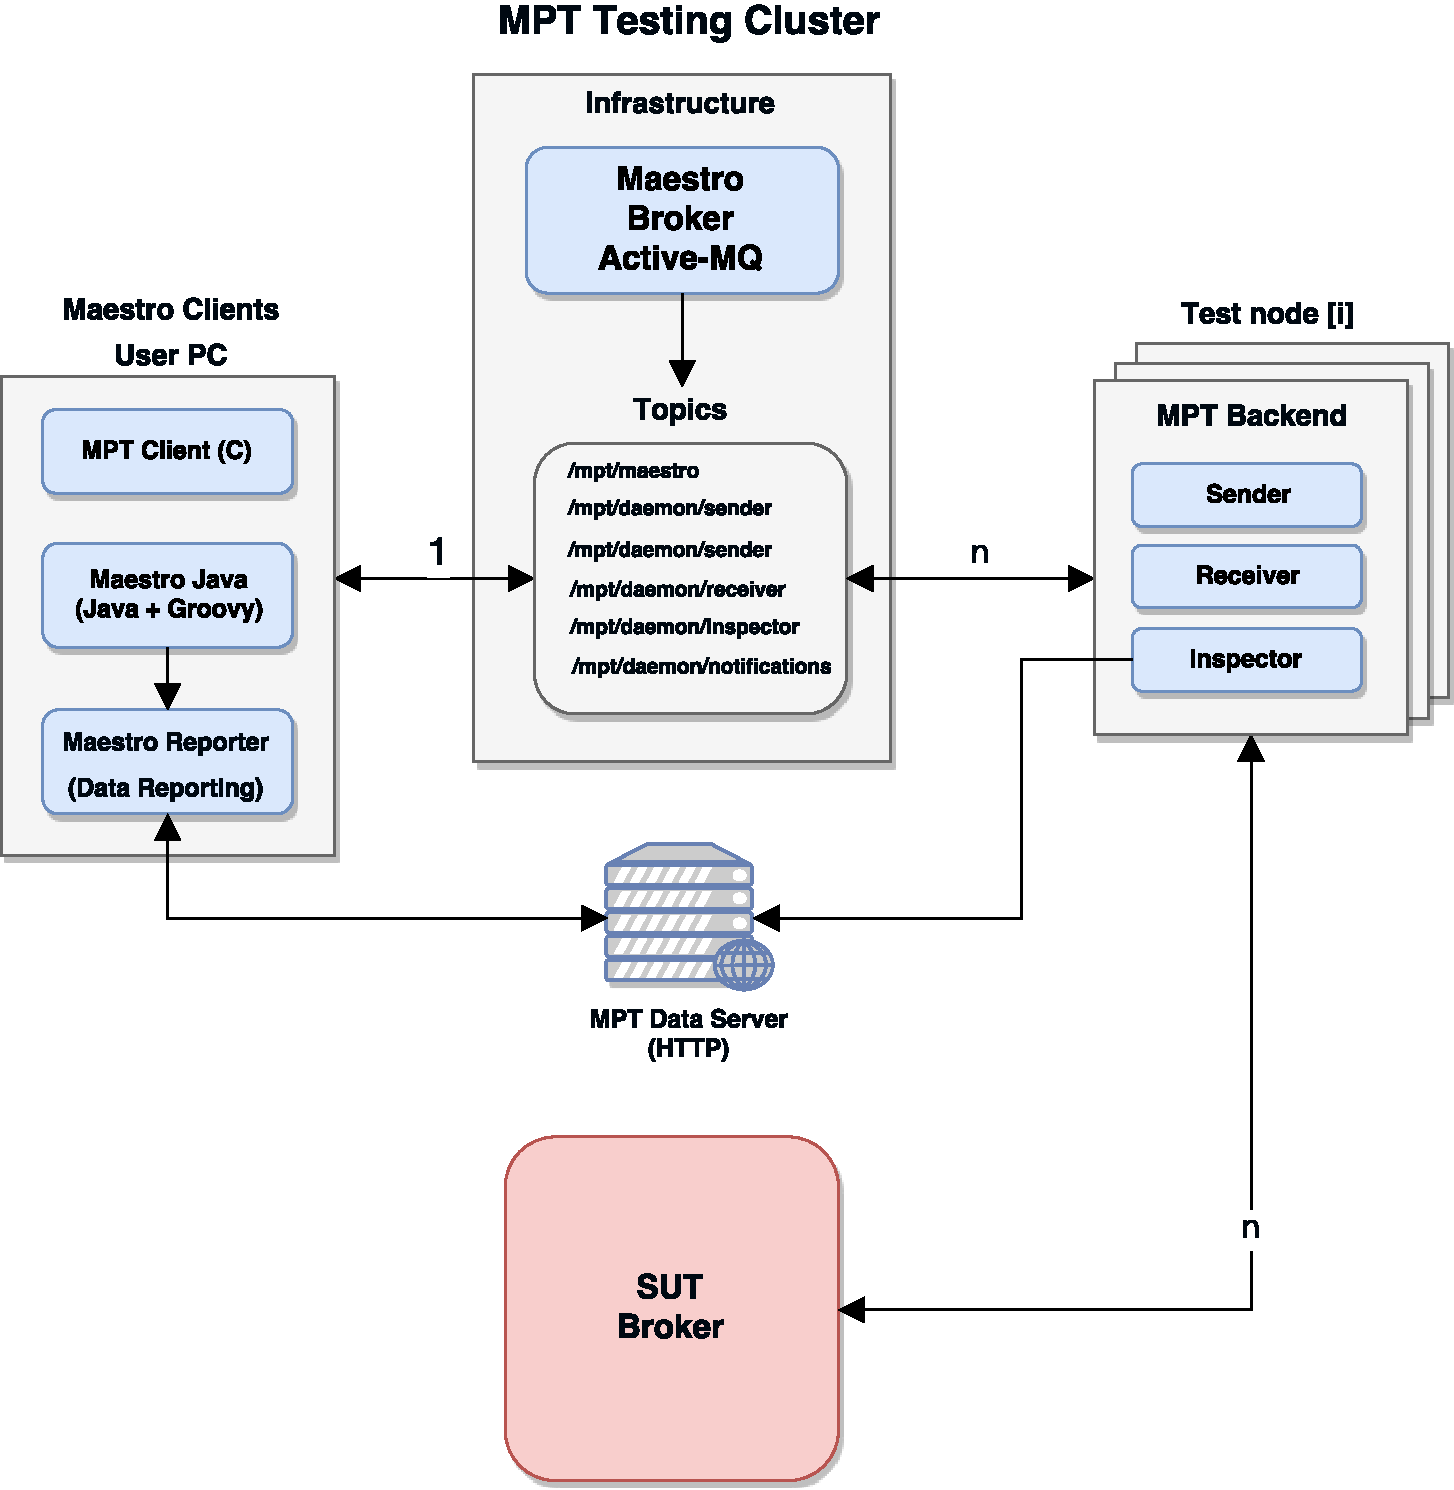
\includegraphics[width=1\linewidth]{msg_perf_tool.pdf}
	\caption{Scheme of communication and protocols used between the Messaging Performance Tool and testing nodes.}
	\label{fig:maestro}
\end{figure}

The actual communication between components during the test cases is realized using the Maestro Protocol\,---\,a binary protocol implemented on top of the MessagePack\footnotemark{}. For the message exchange between nodes it currently uses MQTT protocol (version 3.1.1) and for sending the testing data to data server it uses HTTP protocol (version 1.1). The messages exchanged between the peers are called notes. In the Figure \ref{fig:maestro} you can see the scheme of communication between the Maestro and testing nodes\footnote{Image source\,---\,\url{https://github.com/maestro-performance/msg-perf-tool/blob/master/doc/maestro-overview.png}}. The communication between sender/receiver used specific protocols based on client type: AMQP, STOMP and OpenWire protocols. The inspector and the agent communication with SUT is based on send requests to AMQP management interface, which return proper response with specific data. The agent also executes scripts directly on the SUT node.

\footnotetext{Messagepack\,---\,\url{https://msgpack.org/}}

The current version of Maestro offers 17 commands for test setting and execution\footnotemark{}. These are basic commands such as \emph{start receiver}, or \emph{test success notification} without payload. The other group of commands has additional setting (payload) where it can specify the test behavior. Good example is the \emph{set request} which sets all necessary test options (test duration, rate, fail condition and so on). Another command with payload is e. g. \emph{ping request}.

\footnotetext{All commands are available at \url{https://github.com/maestro-performance/msg-perf-tool/tree/master/doc/maestro/protocol}}

\subsection{Metrics}
\label{sec:Metrics}

The type of metrics collected during tests depends on the component. In the Table \ref{tab:maestro_metrics} you can see the summary of the metrics, which are collected for each component. Metrics for Broker component are collected by the Inspector, which is strictly bounded only to one node with SUT.


\begin{table}[h]
\caption{The summary of Maestro metrics collected during the performance test cases.}
\centering
\begin{tabular}{|p{2.5cm}|p{3.5cm}|p{7cm}|}
\hline
\rowcolor[HTML]{C5E3DF}
\multicolumn{1}{|c|}{\textbf{Component}} & \multicolumn{1}{c|}{\textbf{Metrics}} \\ \hline
\textbf{Sender}                          & Throughput                            \\ \hline
\textbf{Receiver}                        & Throughput                            \\ \hline
\textbf{}                                & Latency                               \\ \hline
\textbf{Broker}			                		 & JVM heap memory                       \\ \hline
                                         & JVM non-heap                          \\ \hline
                                         & Broker internals                      \\ \hline
                                         & OS basic memory                       \\ \hline
                                         & OS resources                          \\ \hline
 \textbf{Router}			                	 & Memory statistics                     \\ \hline
 											                	 & Network neighbors information    \\ \hline

\end{tabular}
\label{tab:maestro_metrics}
\end{table}


%--------------------------------------------------------
%--------------------------------------------------------
%--------------------------------------------------------
%--------------------------------------------------------
\section{Maestro-Agent Extension}
\label{sec:maestro_agent}
The current version of Maestro however cannot use all performance testing and network recovery capabilities of the Qpid-Dispatch. For better performance analysis and measurements it is necessary to design and implement additional functionality for the MPT. We propose a new component called Maestro-agent designed for simple execution of user specific scripts on testing nodes. However, Maestro is not a simple project, so creating new handlers for some testing purpose can be difficult. Hence, creation of Maestro-agent offers an elegant solution, where every user only needs to provide groovy scripts with action descriptions. This way user does not need to change Maestro code at all, he only has to specify the source of the extension point, for example a git repository, which is downloaded by agent and executed during the test scenario.


\begin{figure}[h]
	\centering
	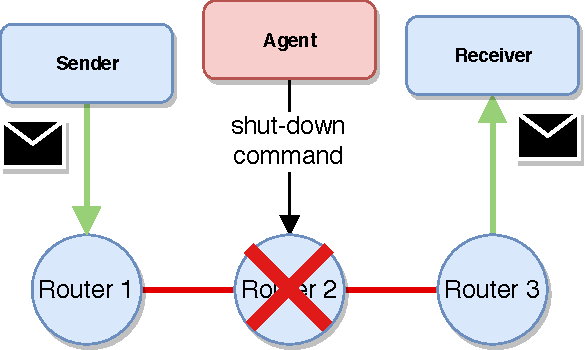
\includegraphics[width=0.9\linewidth]{agent_2_excel.pdf}
	\caption{Example of agent's behavior during the test.}
	\label{fig:agent_2}
\end{figure}

Since we want to measure the performance of Qpid-dispatch during unexpected situations, we will use the main function of the agent to execute the code which will influence the behavior of the network during the test. This way Maestro is able to answer questions such as \emph{"how the crash of one major network devices influence the load?"} or \emph{"how long it takes to network device to recover from overload?"}. An example of agent execution is depicted in the Figure \ref{fig:agent_2}, where the agent shuts down Router\,2 and all of the load is then redirected through the Router\,3.

Basically Maestro-agent will execute external scripts for handle some atomic operation on the specific node. The agent only needs source of this scrips, for example an url for git repository. The agent will download the repository and then execute each script in seperate thread. In this scripts, user can specify when the code should be executed by specify the time of start.

In the Section \ref{sec:experimental_evaluation} I will further show how agent's actions influences the performance of series of graphs.

\begin{figure*}[h!t]
	\centering
	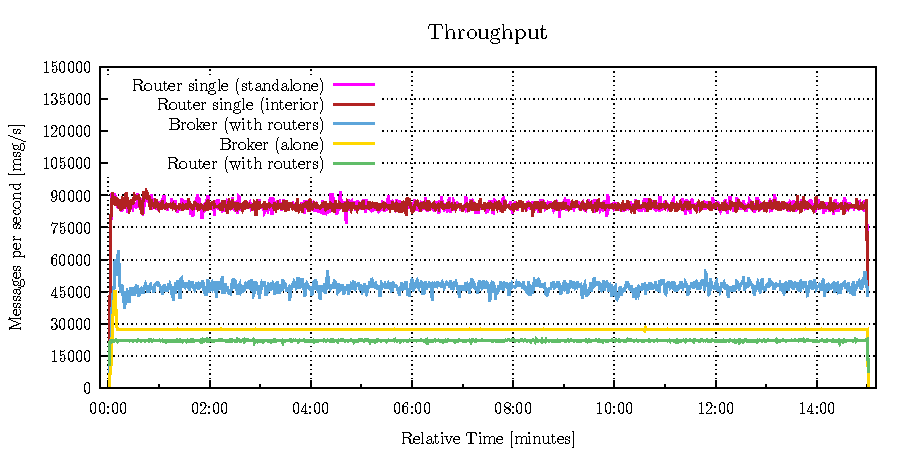
\includegraphics[width=1\linewidth]{results/throughput.pdf}
	\caption{Chart of maximum throughput of router and broker during specific test cases.}
	\label{fig:max_rate}
\end{figure*}

\begin{figure}[h!t]
	\centering
	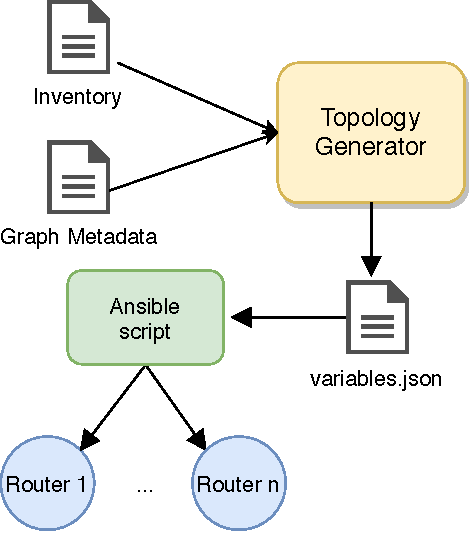
\includegraphics[width=0.5\linewidth]{generator_excel.pdf}
	\caption{Configuration files generation by Topology Generator and deployment by Ansible.}
	\label{fig:generator}
\end{figure}


%--------------------------------------------------------
%--------------------------------------------------------
\section{Topology Generator}
Since we want to run tests with as much automation as possible, I created more auxiliary tools for smoother automatization. One of these is the Topology Generator, which creates network topology configuration files based on users metadata. This is very helpful in cases of bigger networks or frequent changes in topologies. Topology generator expects two files as an input: Inventory with list of nodes and Metadata file with network type and additional settings. The output is a simple JSON file with generated configuration for each router node in the network.

The automatic deployment is realized by Ansible \cite{Ansible} script. Ansible is a simple automation framework which allow users to automate daily tasks on multiple nodes or containers. It offers very simple interface which allows to deploy specific components on each node of the network. During the tests, the Ansible is used for Maestro and network topology deployment. In case of topology deployment, Ansible script load and fill a template for Qpid-dispatch configuration file and fills it up with data from generator output. Ansible then ensures that each node has proper configuration settings. The main functionality of Topology Generator and Ansible deployment scripts is depicted on the Figure \ref{fig:generator}



%--------------------------------------------------------
%--------------------------------------------------------
\section{Experimental Evaluation}
\label{sec:experimental_evaluation}

Since Maestro works as the orchestration system, I needed proper infrastructure before I could run any test for our experimental evaluation. The architecture of Maestro, described in Section \ref{sec:MessagingPerformanceTool}, specifies that in ideal scenario I need at least four machines for running a simple test: maestro broker, sender, receiver, and SUT. The amount of needed machines rises with more complex scenarios and larger network and this process is not comfortable to deploy all of this manually. Here I use the Ansible script with the data generated from Topology Generator. I conducted the following experiments with our extension of the MPT tool to demonstrate its capabilities. I created a simple topologies of three routers connected together in line and compared it with topology of router, broker and router connected in line as well. Example of only router configuration is depicted in the Figure \ref{fig:agent_2}. For both of these configurations I compared the throughput and latency of these combinations and discuss the results with supervisors and author of MPT. The experiment show, that extended MPT can significantly help to test various scenarios and network behaviours.

\subsection{Throughput}
\label{Throughput}

\begin{figure*}[h!t]
	\centering
	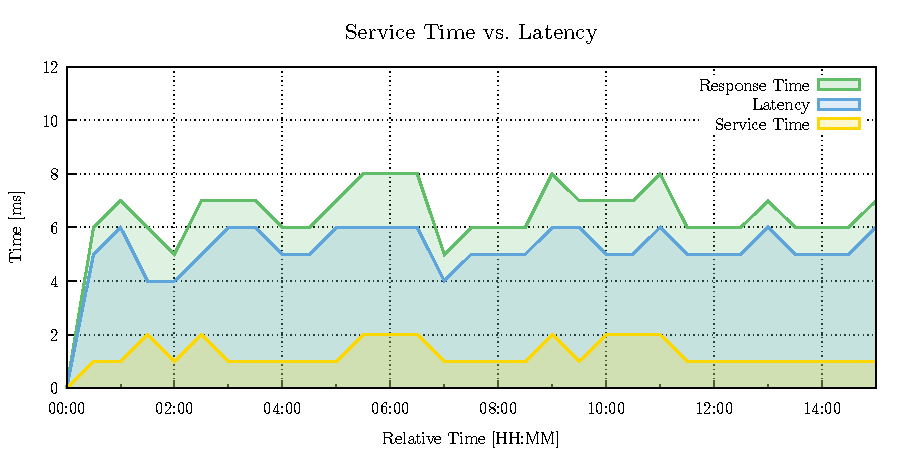
\includegraphics[width=1\linewidth]{results/latency.pdf}
	\caption{Latency chart showing the difference between router and broker latency at 80\,\% of maximum rate. The router's latency is significantly better than latency of Broker.}
	\label{fig:latency}
\end{figure*}

I measured throughput only by load generators\,---\,\emph{Maes\-tro Sender} and \emph{Maestro Receiver}. Load generation depends on the test properties. Maestro is able to create unbounded rate test, during which it generates as much load as it can. This type of test was used to reach maximum handled rate of Qpid-dispatch and its result is depicted in the Figure \ref{fig:max_rate}. However, the maximum rate was not achievable on all topology types. Qpid-dispatch offers two modes\,---\,\emph{standalone} and \emph{interior}, where standalone works as single router machine in the network, while interior type works with multiple routers. The current version of Qpid-dispatch has an ability to load balance when buffers are almost full. This ability offers faster message delivery in cost of a slower throughput. I compared standalone and interior router as depicted in the Figure \ref{fig:max_rate} as the first case study.

But, throughput can be influenced by other network devices. As you can see in the Figure \ref{fig:max_rate}, the lone router (pink and red color) can reach around 90\,000 messages per second, while lone broker reaches only about 30\,000 messages per second. However, when I try to add another component, the throughput changes significantly. The topology with three routers uses the flow-control of interior setting which cause perceptible throughput degradation of that network (shown by green color). On the other hand, when I replace router in the middle by broker, the throughput is raised to 50\,000 messages per second. Thus you can see that load balancer of Qpid-dispatch should be improved, because throughput degradation is too high as I demonstrated. However, It has to be said that high throughput does not necessarily mean better performance. I discuss this in the Subsection \ref{Latency}.

\subsection{Latency}
\label{Latency}

\begin{figure*}[h!t]
	\centering
	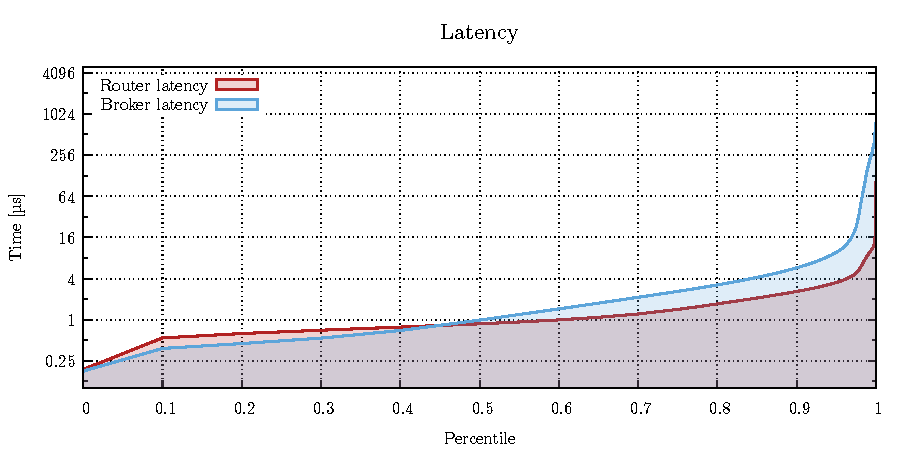
\includegraphics[width=1\linewidth]{results/latency_single.pdf}
	\caption{Router and broker latency comparison during the same load. You can see that router's latency is more stable than latency of Broker.}
	\label{fig:latency_single}
\end{figure*}

Latency is measured only by Maestro Receiver from certain load samples. Since the Broker is a distribution service, which needs to store messages for some time, or create and keep queues for clients, it has higher requirements for system resources. On the other hand Qpid-dispatch has only one purpose\,---\,to route the messages. This makes it more faster than the Broker. So high load can be unprofitable, especially in the case of topology with broker. The broker can handle less messages than router, but using router can raise broker's throughput since it can control the load. Thus gives more time to broker to process messages even with higher load.

In the Figure \ref{fig:latency} you can see the latency difference that I measured between those two services. You can see the measured latency on specified topology of three routers (red), and two routers with some middle-broker (blue). The latency curve proves, that router is able to deliver messages into its destination faster than broker, because broker needs to store them in the memory. The latency of the topology with broker reaches more than 1\,000\,$\mu$s; on the other hand, topology consisting of routers has significantly better latency that tops around 256\,$\mu$s. The important thing is, that both of those tests were run on the same machines and with the same test setting: 10\,000\,000 messages, 80\% of maximum rate with five parallel senders and receivers and 256 byte message size.


Another interesting comparison is between the latency of single instance router and broker. In the Figure~\ref{fig:latency_single} you can see the latency output from the test with the same load of 70\,000 messages per second. Broker can reach this rate with additional queue settings. This configuration improves the distribution of incoming load between multiple queues. That causes that Broker is slightly faster than the router in 40\% cases, but even with that, router is faster in other cases. Router latency has threshold around 60\,$\mu$s, while Broker's has threshold over 1\,000\,$\mu$s. The conclusion is, that router should be much faster than Broker during certain circumstances.

\subsection{Agent Evaluation}
Moreover, I will present some preliminary results with using the agent extension and changing behavior of topology depicted in the Figure \ref{fig:agent_2}. In the Figure \ref{fig:agent_throughput} you can see throughput of few simple tests during which middle router is restarted or shut down. The throughput spikes are caused by these events. Since router does not have any queues to store messages, the messages are then discarded and lost. However, the sender does not receive acknowledgment of lost messages so it is not router responsibility. In the Table \ref{tab:agent} you can see the duration of each executed operation and rate of lost messages during the operation (with expected amount of messages being 10\,000\,000). For example during the restart, router was completely shutdown for a second during which no messages arrived. However, after the restart there was some time to balance the load to the previous point. This leads to message lost equals to 2 seconds rate.

% Please add the following required packages to your document preamble:
% \usepackage[table,xcdraw]{xcolor}
% If you use beamer only pass "xcolor=table" option, i.e. \documentclass[xcolor=table]{beamer}
\begin{table}[h]
\centering
\caption{Summarization of lost messages during the connection issues.}
\label{my-label}
\begin{tabular}{|c|r|r|}
\hline
\rowcolor[HTML]{C5E3DF}
Operation     & Duration (seconds) & Message Lost \\ \hline
None          & 0        & None         \\ \hline
Restart       & 1        & 46437        \\ \hline
Shutdown      & 12       & 280572       \\ \hline
Long Shutdown & 89       & 1304451      \\ \hline
\end{tabular}
\label{tab:agent}
\end{table}

The Figure \ref{fig:agent_throughput} also shows, that test case with long shutdown is longer about 10 seconds that other scenarios and the throughput after the shutdown is quite higher. This means that router high throughput to even the messages lost.

\begin{figure*}[h!t]
	\centering
	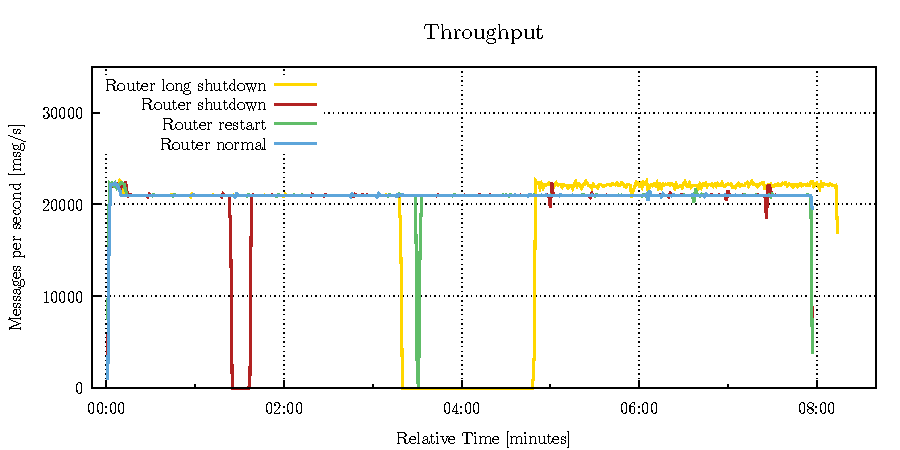
\includegraphics[width=1\linewidth]{results/agent.pdf}
	\caption{Router throughput comparison during the same load after different unexpected events.}
	\label{fig:agent_throughput}
\end{figure*}

Latency of test cases cases with the agent function demonstration is depicted in the Figure \ref{fig:agent_latency}. You can see that router is able to even the latency during the restart and short shutdown with test run without any unexpected behavior. On the other hand, long shutdown (red) gets worse latency almost for 50 percentile of messages.

\begin{figure*}[h!t]
	\centering
	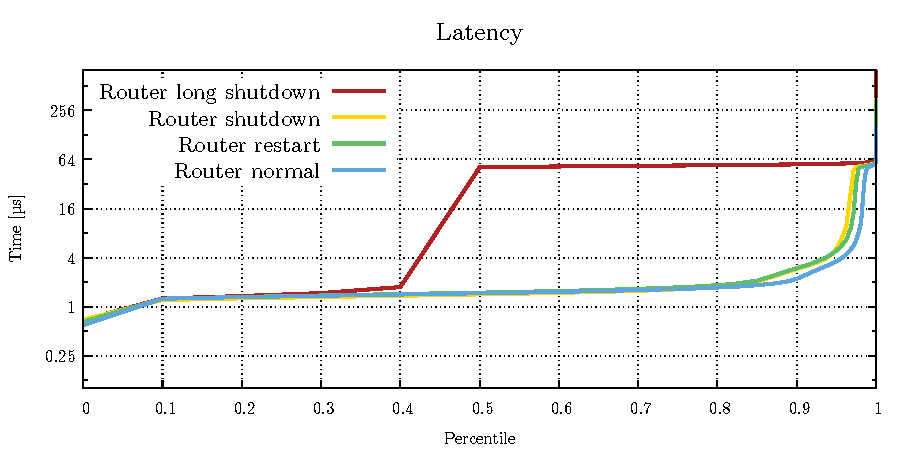
\includegraphics[width=1\linewidth]{results/agent_latency.pdf}
	\caption{Router and broker latency comparison during the same load.}
	\label{fig:agent_latency}
\end{figure*}


%--------------------------------------------------------
%--------------------------------------------------------
%--------------------------------------------------------
\section{Conclusions}
\label{sec:Conclusions}

In this paper, I introduced Messaging Performance Tool and proposed improvements, necessary to extend the capabilities of performance testing of wider range of components. The main improvement is the new extension of MPT, which allows one to run external code during the test. This ability enables behavioral testing of MOM, such as the network service recovery time during the crash, root device crash influence over the topology, or influence of configuration changes made on the fly. The other improvement is the development of Topology Generator, which can significantly simplify the process of test automation.

I evaluated created solution on series of experiments with Qpid-dispatch and Messaging Broker; Maestro is however fully compatible with any other messaging services. This shows wide application for developers who want to test performance of their messaging systems, different topologies or different components.


\section*{Acknowledgements}
I would like to thank my supervisors, Ing. Tomáš Fiedor and Ing. Zdeněk Kraus for their time. Also I would like to thank my colleague and author of Maestro, Bsc. Otavio Rodolfo Piske for his help and guidance during the development and testing. This work is realized in cooperation with Red Hat Czech, s.r.o.

%--------------------------------------------------------
%--------------------------------------------------------
%--------------------------------------------------------
%	REFERENCE LIST
%--------------------------------------------------------
%--------------------------------------------------------
\phantomsection
\bibliographystyle{unsrt}
\bibliography{2018-ExcelFIT-MaestroPerformance-bib}

%--------------------------------------------------------
%--------------------------------------------------------
%--------------------------------------------------------
\end{document}
